\section{The Analogy of City Exploration}

Since to solve is to search, searching is basically exploring your searchable area.

You start with a newly assigned treasure hunt game. You start you search by going through the known routes, following the familiar signposts, try the nearby stores to save your energy, you find a famous gathering place like a museuem or a park.

You start to find the easter egg by visiting the hinted places, and you get there by some known and familiar routes, you can search nearby the hinted places, since you know how to get there and assume you can find there will be considered as being lucky. Sometimes you have to find your own routes by noticing the signposts. And since you might visit the city multiple times, you will gradually remember the notable objects. When you on a road, you will automatically complete the routes without thinking or even chatting with others, until a puzzled crossroad is encountered.

Let's compare the solving route as how much roads you have to travel. And the fluency of your technique mastering is a value of resistance, low value with well trained, and high for poor practice. That might be the case in our brain that the smooth of a chunk is basically the electric current with higher value. And the brain choose load through those low resistance route to save computation energy.

\begin{figure}
  \centerline{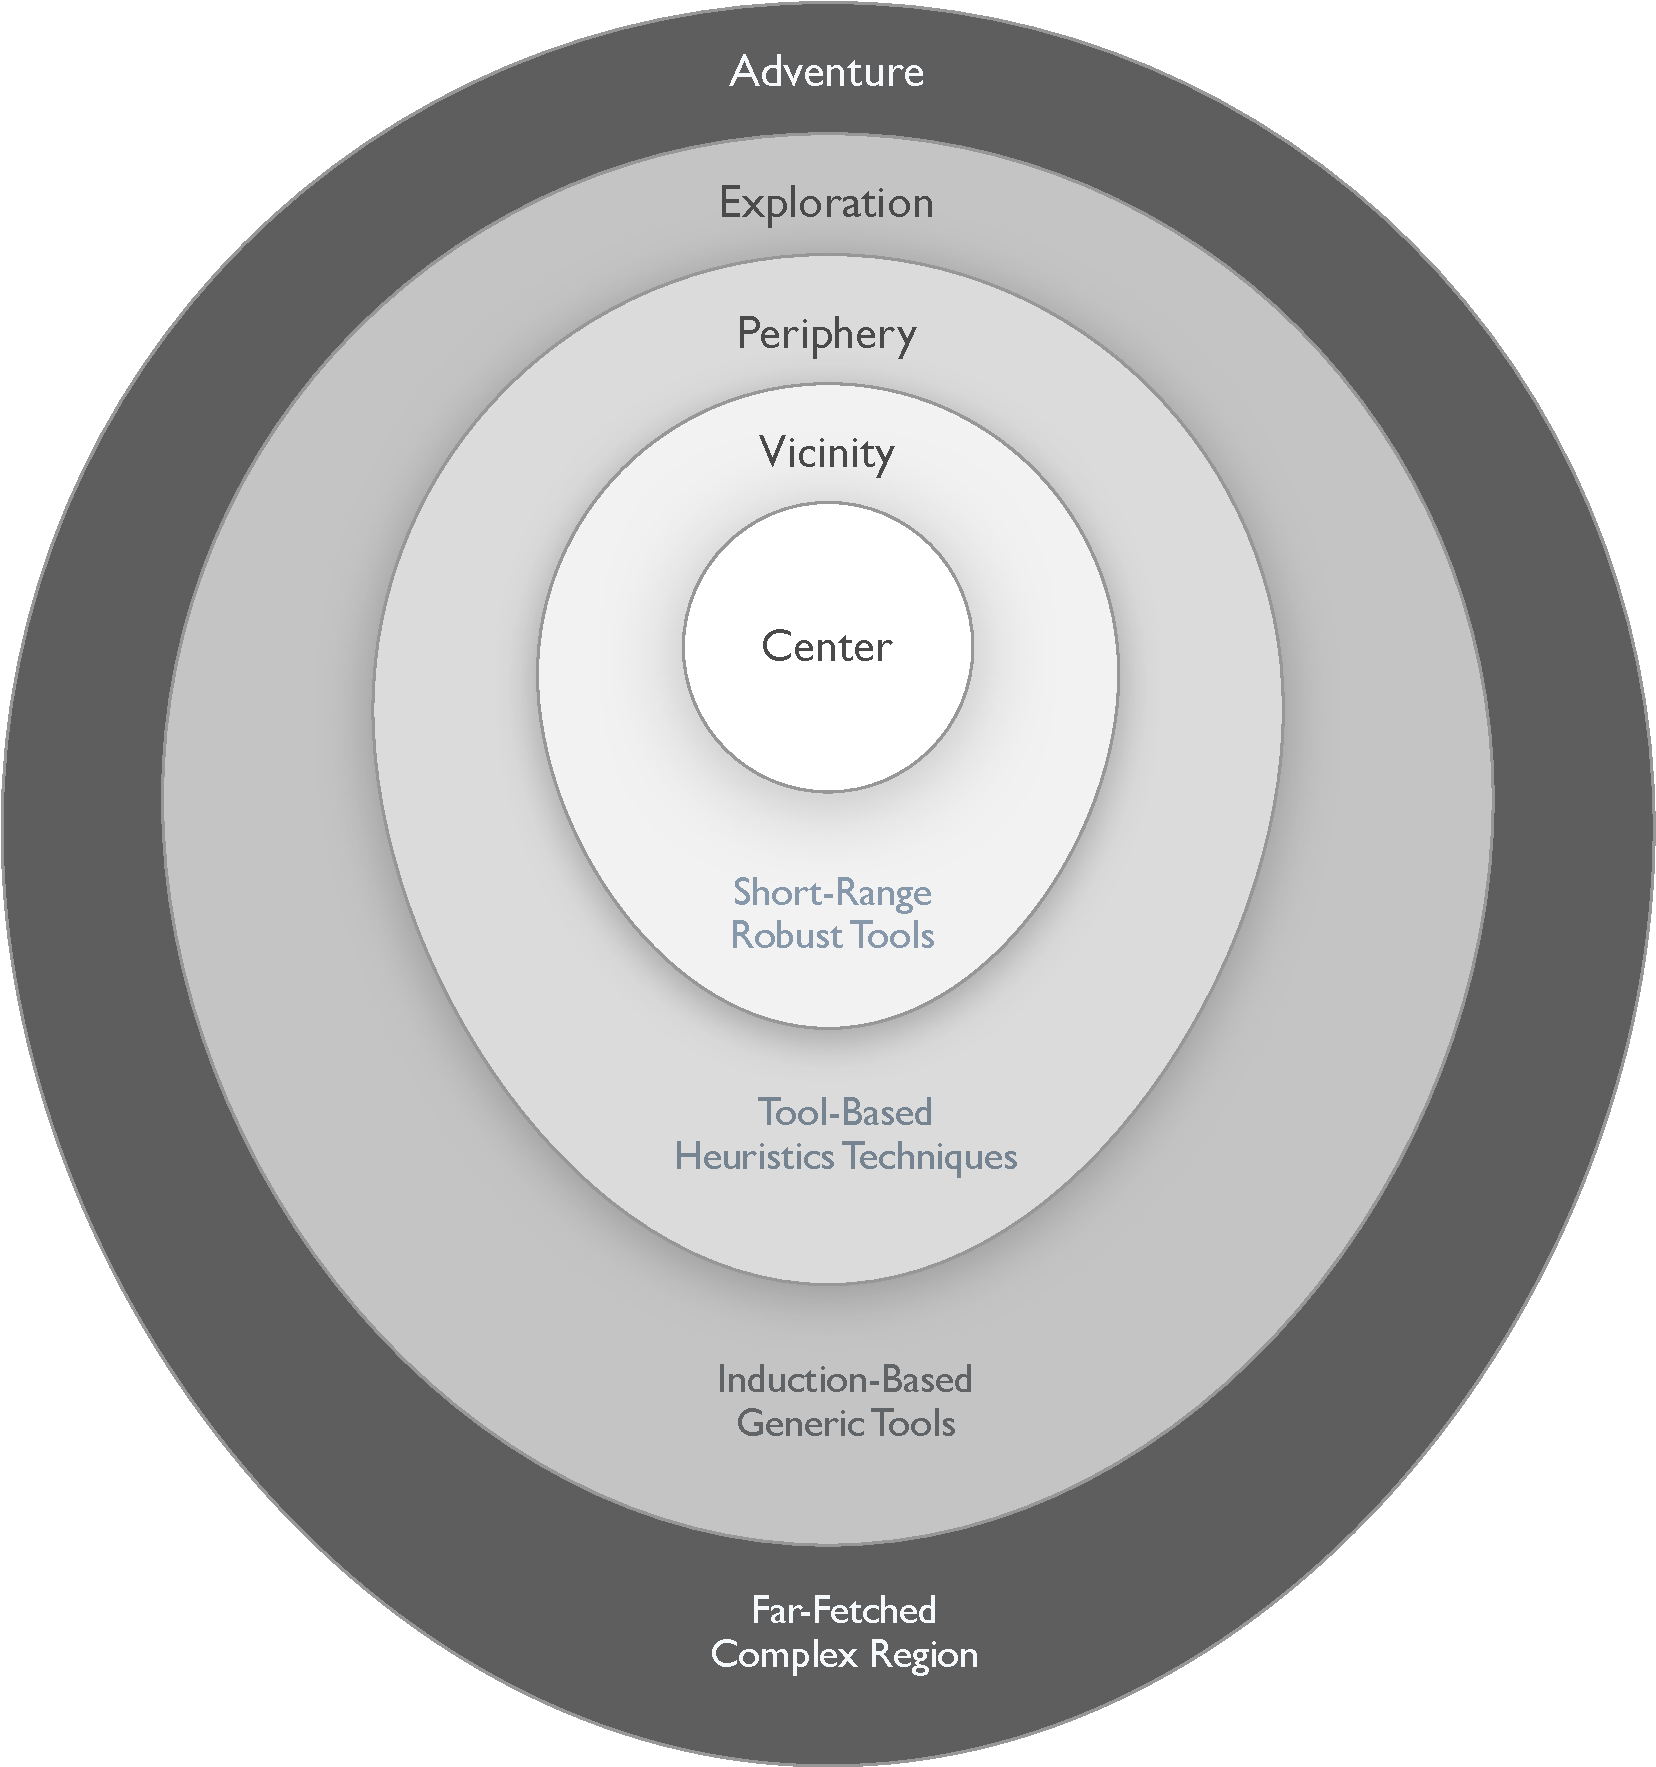
\includegraphics[width=1.2\linewidth]{img/range.pdf}}
  \caption{Types of Transformation}
  \label{fig:range}
\end{figure}
